\documentclass[border=10pt]{standalone}

\usepackage{tikz}
\usepackage{tikzsymbols}
\usetikzlibrary{calc,patterns,shapes.geometric}

\def\centerarc[#1](#2)(#3:#4:#5){\draw[#1] ($(#2)+({#5*cos(#3)},{#5*sin(#3)})$) arc (#3:#4:#5);}

\begin{document}
	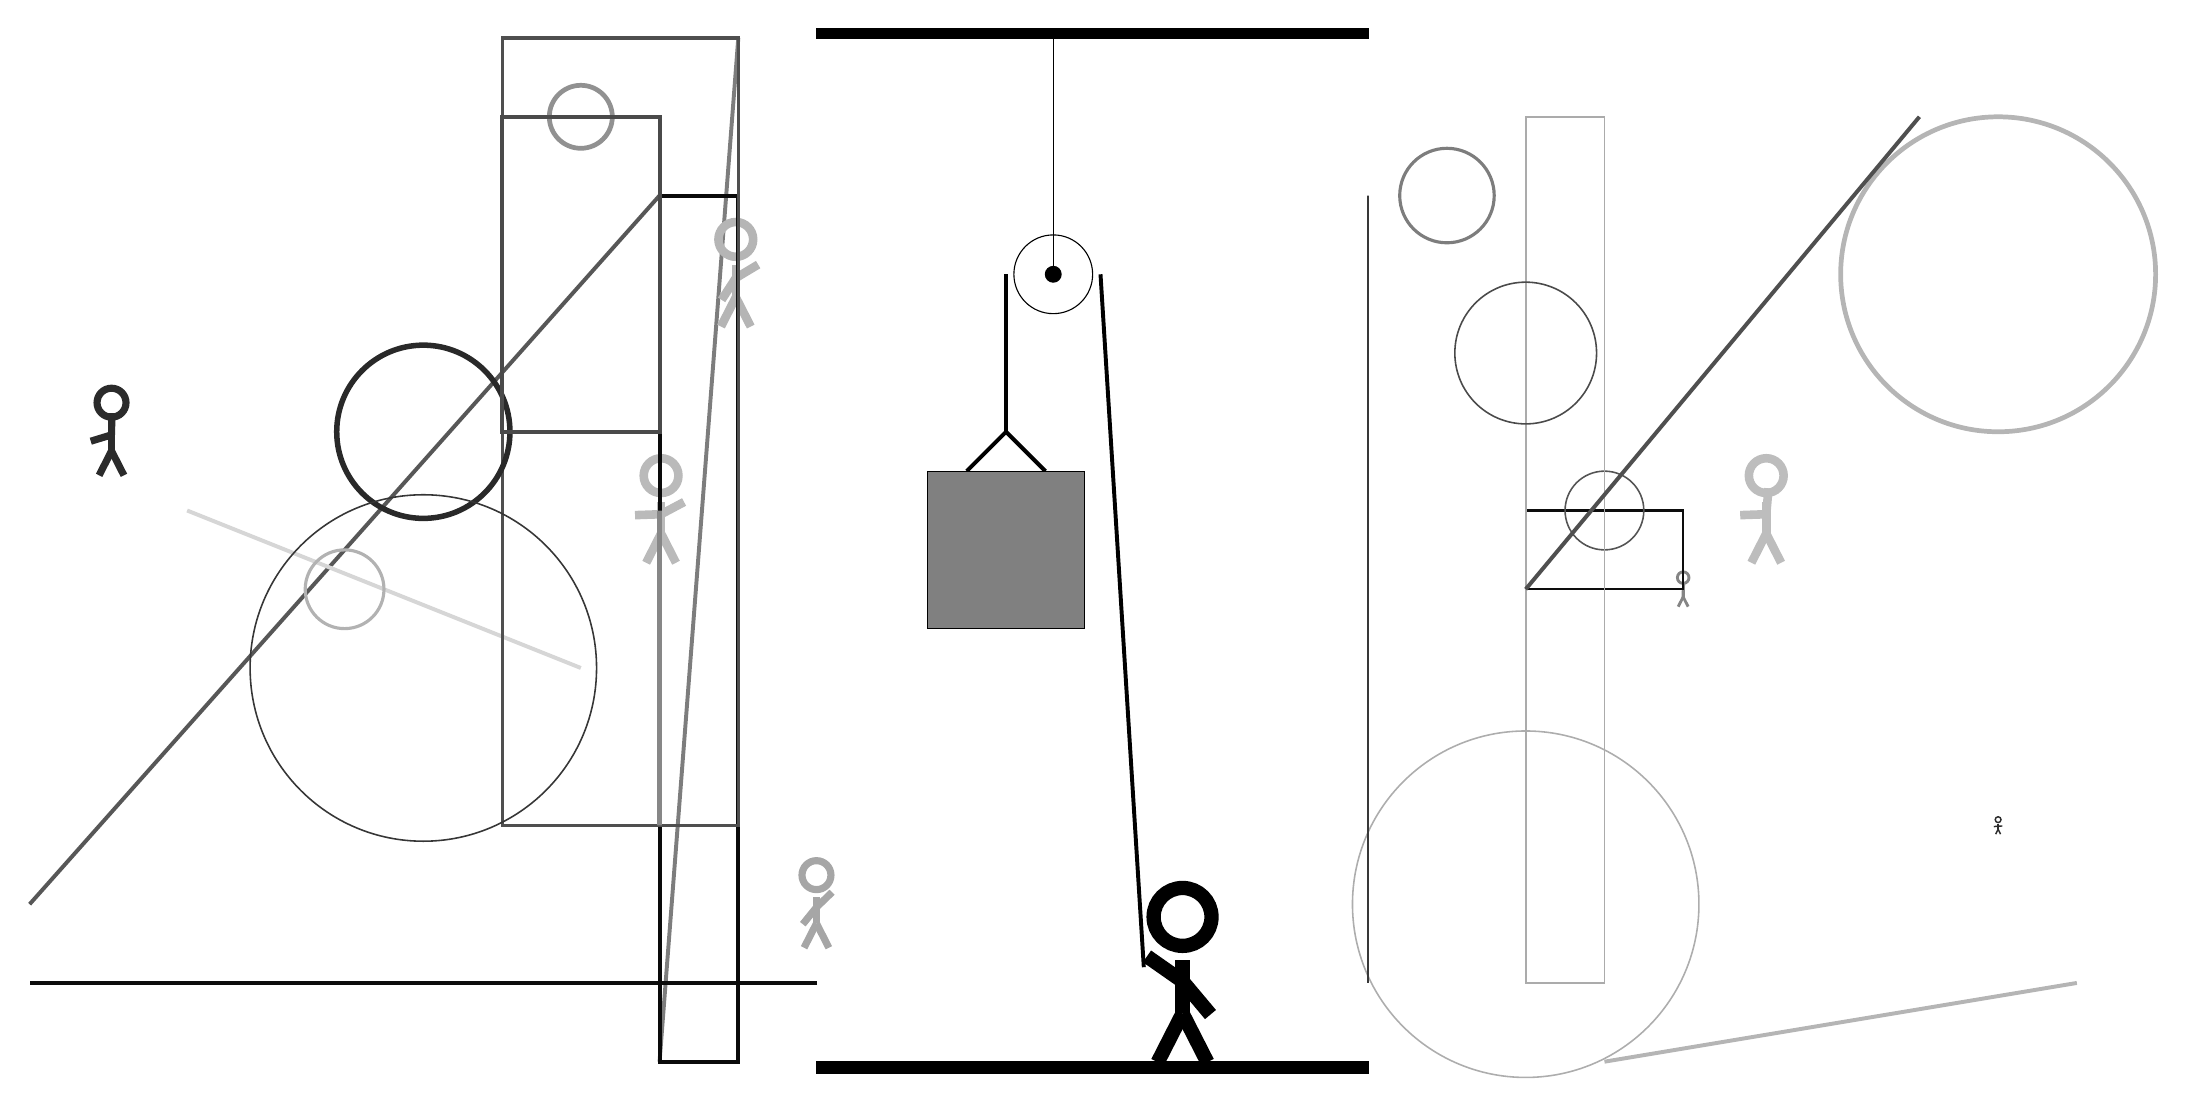
\begin{tikzpicture}
		%%%%% START %%%%%
		
		\draw[fill=black] (-2, 10) rectangle (5, 10.125);
		
		\draw[line width=0.5mm, color=black!66](-4, 8) -- (-12, -1);
		
		\node[line width=0.2mm, color=black!48] at (9, 3) {\Strichmaxerl[2][89][85]};
		\node[line width=0.3mm, color=black!27] at (-4, 4) {\Strichmaxerl[6][2][28]};
		\node[line width=0.3mm, color=black!83] at (-11, 5) {\Strichmaxerl[5][17][89]};
		\draw[line width=0.5mm, color=black!51](-4, -3) -- (-3, 10);
		\draw [line width=0.2mm, color=black!32](7, -1) circle (2.2);
		
		\node[line width=0.6mm, color=black!29] at (-3, 7) {\Strichmaxerl[6][57][31]};
		\draw[line width=0.3mm, color=black!95] (7, 4) rectangle (9, 3);
		\draw[line width=0.5mm, color=black!16](-5, 2) -- (-10, 4);
		
		\draw[line width=0.2mm, color=black!69] (-3, 2) rectangle (-3, -3);
		\draw [line width=0.2mm, color=black!67](8, 4) circle (0.5);
		\draw[line width=0.5mm, color=black!29](8, -3) -- (14, -2);
		\draw[line width=0.5mm, color=black!95](-2, -2) -- (-12, -2);
		
		\draw[line width=0.5mm, color=black!96] (-3, -3) rectangle (-4, 8);
		\draw [line width=0.6mm, color=black!29](13, 7) circle (2.0);
		\draw[line width=0.2mm, color=black!33] (7, 9) rectangle (8, -2);
		
		\node[line width=0.5mm, color=black!26] at (10, 4) {\Strichmaxerl[6][2][85]};
		\draw[line width=0.4mm, color=black!69] (-3, 0) rectangle (-6, 10);
		\draw [line width=0.4mm, color=black!30](-8, 3) circle (0.5);
		\draw [line width=0.4mm, color=black!51](6, 8) circle (0.6);
		\draw [line width=0.7mm, color=black!84](-7, 5) circle (1.1);
		
		\node[line width=0.7mm, color=black!83] at (13, 0) {\Strichmaxerl[1][7][1]};
		
		\draw [line width=0.6mm, color=black!43](-5, 9) circle (0.4);
		\draw[line width=0.5mm, color=black!69](7, 3) -- (12, 9);
		\node[line width=0.3mm, color=black!35] at (-2, -1) {\Strichmaxerl[5][51][44]};
		\draw [line width=0.2mm, color=black!71](7, 6) circle (0.9);
		\draw[line width=0.6mm, color=black!47] (-4, 0) rectangle (-4, 4);
		\draw [line width=0.2mm, color=black!79](-7, 2) circle (2.2);
		
		\draw[line width=0.5mm, color=black!71] (-4, 5) rectangle (-6, 9);
		\draw[line width=0.2mm, color=black!78] (5, -2) rectangle (5, 8);
		
		\draw (1, 7) circle (0.5);
		\draw[fill=black] (1, 7) circle (0.1);
		\draw (1, 10) -- (1, 7);
		
		\draw[line width=0.5mm] (-0.1, 4.5) -- (0.4, 5.0) -- (0.9, 4.5);
		\draw[fill=black!50] (-0.6, 4.5) rectangle (1.4, 2.5);
		
		\draw[line width=0.5mm] (0.4, 7) -- (0.4, 5.0);
		\centerarc[line width=0.5mm](1, 7)(0:180:0.6);
		\draw[line width=0.5mm](1.6, 7) -- (2.15, -1.8);
		
		\node at (2.6, -1.9) {\Strichmaxerl[10][-35][-50]};
		
		\draw[fill=black] (-2, -3) rectangle (5, -3.15);
		
		%%%%% END %%%%%
	\end{tikzpicture}
\end{document}